\documentclass{beamer}
%[handout] option gets rid of extra frames
%\hypersetup{colorlinks=true,
%linkcolor=blue,
%citecolor=red,
%urlcolor=red,
%}
%\usetheme{Darmstadt}
%\usetheme{default}
\usetheme{Boadilla}
 %\usetheme{Madrid}
% \usetheme{Montpellier}
% \usetheme{Warsaw}
% \usetheme{Copenhagen}
% \usetheme{Goettingen}
% \usetheme{Hannover}
%\usetheme{Berkeley}
\numberwithin{equation}{section}
\setbeamertemplate{footline}[page number]{}
\usepackage{lmodern}
\usepackage{tikz}
\synctex=1

%\setlength{\parindent}{0in} %no indentation of paragraphs after section title
%
\newcommand{\rr}{\mathbb{R}}
\newcommand{\p}{\partial}
\newcommand{\zz}{\mathbb{Z}}
\newcommand{\cc}{\mathbb{C}}
\newcommand{\ci}{\mathbb{T}}
\newcommand{\tor}{\mathbb{T}}
\newcommand{\ee}{\varepsilon}
\newcommand{\wh}{\widehat}
\newcommand{\weak}{\rightharpoonup}
\newcommand{\vp}{\varphi}
%
%
\newtheorem{proposition}{Proposition}
\newtheorem{claim}{Claim}
\newtheorem{remark}{Remark}
\newtheorem{conjecture}[subsection]{conjecture}

%%%%%%%%%%%%%%%%%%%%%%
%
\date{}
\title{H\"older Continuity of the Data to Solution Map for HR in the
Weak Topology}
\author{David Karapetyan}
\institute{University of Notre Dame}
\begin{document}

\begin{frame}
    \titlepage
\end{frame}


%\section*{Table of Contents}
%\setcounter{section}{0}
%\begin{frame}
        %\frametitle{Table Of Contents}
            %\tableofcontents
        %\end{frame}

        \begin{frame}
            \frametitle{Introduction}
We consider the hyperelastic rod (HR) Cauchy problem
\begin{gather*}
 \p_t u =  -\gamma u \p_x u -
 \p_{x} (1 - \p_{x}^{2})^{-1} \left[ \frac{3-\gamma}{2}u^2 +
\frac{\gamma}{2} \left( \p_x u \right)^2
\right], \ \gamma \neq 0,
\label{hyperelastic-rod-equation}
\\
 u(x,0) = u_0(x), \; \; x \in \rr, \; \; t \in \rr
\label{init-cond}
\end{gather*}
\begin{itemize}
    \item
        \pause
        Derived by Dai \cite{Dai_1998_Model-equations} as a one-dimensional 
        model for finite-length and
        small-amplitude axial deformation waves in thin cylindrical
        rods composed of a compressible Mooney-Rivlin
        material. The derivation relied upon a reductive perturbation technique.
    \item 
       \pause 
        Well-posedness in $H^{s}$, $s > 3/2$ shown by Yin
        \cite{Yin_2003_On-the-Cauchy-p} and Zhou
        \cite{Zhou_2005_Local-well-pose} for line and circle.
    \item 
       \pause 
        Alternative proof of well-posedness using Galerkin method
outlined in Taylor \cite{Taylor_1991_Pseudodifferent} shown by Karapetyan \cite{Karapetyan:2010fk}. 
\item 
   \pause 
    Special Feature: Unlike KDV, admits peakon ($\gamma > 0$) and cusped
    solutions ($\gamma \neq 0$).
\end{itemize}
\end{frame}
\begin{frame}
Following Chen, Liu, and Zhang \cite{Chen:2011fk} we show the
following result:


\begin{theorem}

\label{thm:main-thm}
For $\gamma \neq 0$, the
data to solution map for HR is H\"older continuous from $B_{H^{s}}(R)$ (in
the topology of $H^{r}$) to $C([0, T], H^{r})$, where $T = T(R)$, for $s >
3/2$, $-1 \le r < s$. More
precisely, consider the following sets 

  
  \begin{equation*}
  \begin{split}
      & \Omega_{1} = \left\{ (s, \ r) \in \rr^{2}:
     \ s>3/2, \ -1 \le r \le s-1, \ s + r \ge 2  \right\}
    \\
    & \Omega_{2} = \left\{ (s, \ r) \in \rr^{2}:
     \ s>3/2, \ -1 \le r < 2-s \right\}
    \\
    & \Omega_{3} = \left\{ (s, \ r) \in \rr^{2}:
    \  s>3/2, \  s-1 < r < s  \right\}.
    \end{split}
\end{equation*}
\end{theorem}
\end{frame}
\begin{frame}
\begin{theorem}
\begin{center}
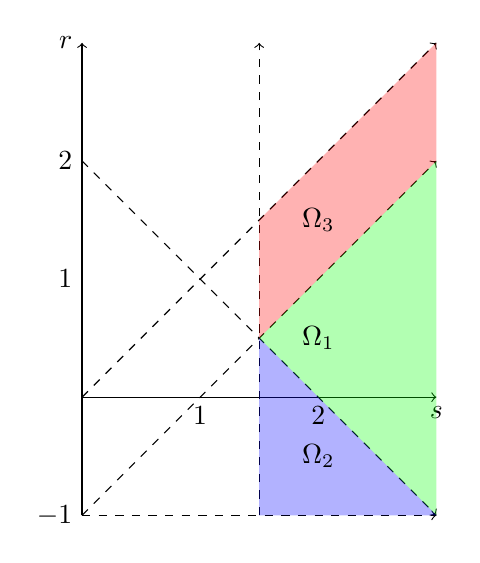
\begin{tikzpicture}[scale=1.5]
Draw thin grid lines with color 40% gray + 60% white

Draw x and y axis lines
\draw [->] (0,0) -- (3,0) node [below] {$s$};
\draw [->] (0,-1) -- (0,3) node [left] {$r$};
\draw [->, dashed] (0,0) -- (3,3);
\draw [->, dashed] (0,-1) -- (3,2);
\draw [->, dashed] (0,2) -- (3,-1);
\draw [->, dashed] (0,-1) -- (3,-1);
\draw [->, dashed] (3/2,-1) -- (3/2, 3);
\fill[color=green, fill opacity=0.3] (1.5, 0.5) -- (3,2) -- (3,0) -- (3,-1);
\fill[color=red, fill opacity=0.3] (1.5, 0.5) -- (1.5,1.5) -- (3,3) -- (3,2);
\fill[color=blue, fill opacity=0.3] (1.5, 0.5) -- (1.5, -1) -- (3, -1);


\foreach \x/\xtext in {1, 2}
    \draw[shift={(\x,0)}]  node[below] {$\xtext$};
\foreach \y/\ytext in {-1, 1, 2}
    \draw[shift={(0,\y)}]  node[left] {$\ytext$};
    \draw (2,1.5) node {$\Omega_{3}$};
    \draw (2,0.5) node {$\Omega_{1}$};
    \draw (2,-0.5) node {$\Omega_{2}$};
\end{tikzpicture}
\end{center}


Then for two initial data $u_{0}, v_{0} \in B_{H^{s}}(R)$, there exist unique
corresponding solutions $u(x,t), v(x,t)$ for $0 \le t \le T= T(R)$ to the
HR equation which satisfy 
\end{theorem}
\end{frame}
\begin{frame}
    \begin{theorem}

\begin{equation*}
\begin{split}
  \| u(t) - v(t) \|_{H^{r}} \le C \| u_{0} - v_{0} \|_{H^{r}}^{\alpha(s, r)},
  \quad 0
  \le t \le T
\end{split}
\end{equation*}


where 


\begin{equation*}
\begin{split}
\alpha = 
\begin{cases}
   1, \quad & (s,r) \in \Omega_{1} 
  \\
   2(s-1)/(s-r),  \quad & (s, r) \in \Omega_{2}
  \\
   s-r, \quad & (s, r) \in \Omega_{3}.
\end{cases}
\end{split}
\end{equation*}
\end{theorem}
\pause
\begin{itemize}
    \item
This result improves upon the H\"older continuity result in
\cite{Chen:2011fk} (there it is for $0 \le r < s$) by a full degree in $r$. 
\item Proof in periodic analogous to non-periodic
\end{itemize}

\end{frame}

\begin{frame}


\frametitle{Region $\Omega_{1}$ $(-1 \le r \le s-1, \ s + r \ge 2$)} 

Let $u_{0}(x), v_{0}(x)
\in B_{H^{s}}(R)$, $s > 3/2$ be two initial datum. Then from
the well-posedness theory for HR \cite{Karapetyan:2010fk}, we
know that there exists unique corresponding solutions $u, v \in C(I,
B_{H^{s}}(2R))$ to the HR Cauchy problem.
Set $v=u-w$. Then $v$ solves the Cauchy-problem

\pause
\begin{align*}
& \p_t v
=  -\frac{\gamma}{2} \p_x [v(u + w)] 
\\
\notag
& \phantom{\p_t v = }-\p_x (1 - \p_{x}^{2})^{-1} \left\{
\frac{3-\gamma}{2}[v(u+w)] + \frac{\gamma}{2}[\p_x v \cdot \p_x (u+w)]
\right\},
\\
& v(x,0) = u_{0}(x) - v_{0}(x).
\end{align*}
\end{frame}

\begin{frame}
Let

\begin{equation*}
    D^{m} = (1 - \p_x^2)^{m/2}, \quad m \in \rr.
\end{equation*}

Applying $D^r$ to both sides then 
multiplying both sides by $D^r v$ and integrating, we obtain


\begin{equation*}
\begin{split}
 \frac{1}{2} \frac{d}{dt} \|v\|_{H^r}^2
 = & -\frac{\gamma}{2} \int_{\rr} D^r \p_x [v(u+w)] \cdot
D^r v \ dx
\\
& - \frac{3-\gamma}{2} \int_{\rr}  D^{r -2}
\p_x[v(u+w)] \cdot
D^r v \ dx  
\\
& - \frac{\gamma}{2} \int_{\rr} D^{r 
-2} \p_x [ \p_x v
\cdot \p_x (u+w)]\cdot D^r v \ dx.
\label{2v}
\end{split}
\end{equation*}
\end{frame}


\begin{frame}
\frametitle{Estimate of Integral 1} Note that


\begin{equation*}
\begin{split}
& \left |  -\frac{\gamma}{2} \int_{\rr} D^r \p_x [v(u+w)] \cdot
D^r v \ dx \right |
\\
& =
\left |
-\frac{\gamma}{2} \int_{\rr} \left[ D^r \p_x, \ u+w \right]v \cdot
D^r v \ dx - \frac{\gamma}{2} \int_{\rr} (u+w) D^r
\p_x v \cdot D^r v\ dx
\right | \\
& \lesssim \left |
\int_{\rr} \left[ D^r \p_x, \ u+w \right]v \cdot
D^r v \ dx \right |
+ \left | \int_{\rr} (u+w) D^r \p_x v
\cdot D^r v\
dx \right |.
\label{4v}
\end{split}
\end{equation*}

\pause

Observe that integrating by parts gives


\begin{equation*}
\begin{split}
\left | \int_{\rr} (u+w) D^r \p_x v \cdot
D^r v \ dx \right |
\le \|\p_x (u+w)\|_{L^\infty}
\|v\|_{H^r}^2.
\label{4'v}
\end{split}
\end{equation*}




\end{frame}

\begin{frame}
To estimate the remaining piece, we shall need the following
following result taken from \cite{Himonas:2010p1187}:

    \begin{lemma}[Commutator Estimate]
\label{cor1}
If $s > 3/2$ and $-1 \le r  \le s -1$, then


\begin{equation*}
\begin{split}
\|[D^r \p_x ,f]g\|_{L^2} \le C \|f\|_{H^s} \|g\|_{H^r}.
\label{15}
\end{split}
\end{equation*}


\end{lemma}
\end{frame}

\begin{frame}
Set $s > 3/2$ and $-1 \le r \le s -1$. An application of 
Cauchy-Schwartz and the Commutator Estimate then yields 


\begin{equation*}
\begin{split}
 \left | \int_{\rr} [D^r \p_x, \ u+w] v
\cdot D^r v \ dx \right |
& \lesssim \|u+w\|_{H^s} 
\|v\|_{H^r}^2.
\label{7v}
\end{split}
\end{equation*}


\pause

Combining everything and applying the Sobolev Imbedding 
Theorem, we obtain 


\begin{equation*}
\begin{split}
\left |  -\frac{\gamma}{2} \int_{\rr} D^r \p_x [v(u+w)] \cdot
D^r v \ dx \right |
 \lesssim \|u+w\|_{H^s} \|v\|_{H^r}^2
\label{8v}
\end{split}
\end{equation*}
for $s > 3/2, \ -1 \le r \le s-1$.
\end{frame}

\begin{frame}
\frametitle{Estimate of Integral 2} 

%%%%%%%%%%%%%%%%%%%%%%%%%%%%%%%%%%%%%%%%%%%%%%%%%%%%%


               %frac deriv est


%%%%%%%%%%%%%%%%%%%%%%%%%%%%%%%%%%%%%%%%%%%%%%%%%%%%%


\begin{lemma}[Fractional Sobolev]
For $s > 3/2$, $r \le s$, $s + r \ge 2$, we have


\begin{equation*}
\begin{split}
  \| fg \|_{H^{r-1}} \lesssim \| f \|_{H^{r-1}} \| g \|_{H^{s-1}}.
\end{split}
\end{equation*}


\label{lem:frac-deriv}
\end{lemma}

%\begin{itemize}
    %\item  Improves upon estimate in Himonas and Kenig \cite{Himonas:2009fk}
        %\begin{equation*}
            %\| fg \|_{H^{\sigma -1}} \lesssim \| f \|_{H^{\sigma -1}} \| g
            %\|_{H^{\sigma}}, \quad 1/2 < \sigma < 1
        %\end{equation*}
%\end{itemize}

\end{frame}

\begin{frame}


Applying Cauchy-Schwartz and the Fractional Sobolev Lemma, we obtain



\begin{equation*}
\begin{split}
\left | - \frac{3-\gamma}{2} \int_{\rr}  D^{r -2}
\p_x[v(u+w)] \cdot
D^r v \ dx  \right |
 & \lesssim \|u+w\|_{H^{r -1}} \|v\|_{H^r}^2
\end{split}
\end{equation*}

\pause

which implies
\begin{equation*}
\begin{split}
\left | - \frac{3-\gamma}{2} \int_{\rr}  D^{r -2}
\p_x[v(u+w)] \cdot
D^r v \ dx  \right |
 & \lesssim \|u+w\|_{H^{s}} \|v\|_{H^r}^2
 \label{3v}
\end{split}
\end{equation*}

for $s > 3/2, \ r \le s, \ \text{and} \ s + r \ge 2$.

\end{frame}
\begin{frame}
\frametitle{Estimate of Integral 3} 

Applying Cauchy-Schwartz, the Fractional Sobolev Lemma and the inequality $\| f_{x}
\|_{H^{m-1}} \le \| f \|_{H^{m}}$,  we conclude that

\begin{equation*}
\begin{split}
\left | - \frac{\gamma}{2} \int_{\rr} D^{r 
-2} \p_x [ \p_x v
\cdot \p_x (u+w)]\cdot D^r v \ dx \right | 
 \lesssim \|u+w \|_{H^{s}}
\|v\|_{H^r}^2
\label{3'v}
\end{split}
\end{equation*}


for $s > 3/2, \ r \le s, \ \text{and} \ s + r \ge 2$.
\end{frame}
\begin{frame}
Grouping estimates for Integrals 1-3, get


\begin{equation*}
\begin{split}
\frac{1}{2} \frac{d}{dt}
\|v\|_{H^r}^2
& \lesssim \|u+w\|_{H^s}
\|v\|_{H^r}^2, \quad | t | < T
\\
& \le 4R \| v \|_{H^{r}}^{2}
\label{9v}
\end{split}
\end{equation*}

\pause
which by Gronwall gives

\begin{equation*}
  \label{lip-ineq}
\begin{split}
  & \| u(t) - w(t) \|_{H^{r}} \le C \| u_{0} - w_{0} \|_{H^{r}}, 
  \\
  & \text{for} \ | t | < T,
  \ s > 3/2, \ -1 \le r \le s-1, \ s + r \ge 2.
\end{split}
\end{equation*}

\pause

Hence, in region $\Omega_{1}$, the data to solution map is locally Lipschitz from
$B_{H^{s}(R)}$ (measured with the $H^{r}$
norm) to $C([-T, T], H^{r})$, with Lipschitz constant $C = C(s, r, R)$.

\end{frame}



\begin{frame}
\frametitle{Region $\Omega_{2}$ $(-1 \le r < 2-s)$} 

We have the estimate
\begin{equation*}
  \label{fgh}
\begin{split}
  \| v(t) \|_{H^{r}}
  & < \|v(t) \|_{H^{2-s}}.
    \end{split}
\end{equation*}

\end{frame}
\begin{frame}
We see that Lip inequality is valid for $r = 2-s$, $3/2 < s \le 3$.
Hence, applying it, we obtain 




\begin{equation*}
\begin{split}
\| v(t) \|_{H^{r}}
 \lesssim \|v(0) \|_{H^{2-s}}.
\end{split}
\end{equation*}





We need the following interpolation
result. 
 \end{frame} 

 \begin{frame}
     \begin{lemma}[Interpolation]
  For $m_{1} < m < m_{2}$,
  
  
  \begin{equation*}
  \begin{split}
    \| f \|_{H^{m}} \le \| f \|_{H^{m_{1}}}^{(m_{2}-m)/(m_{2} - m_{1})} \| f
    \|_{H^{m_{2}}}^{(m -m_{1})/(m_{2} - m_{1})}.
  \end{split}
  \end{equation*}
  
  
  
   
  
\label{lem:interp}
\end{lemma}

\pause
Applying the lemma with $m_{1} =r$, $m = 2-s$, and $m_{2} = s$ (notice
$m_{2} > m$ for $s > 1$), we bound 


\begin{equation*}
\begin{split}
    \| v(0) \|_{H^{2-s}} 
    & \le \| v(0) \|_{H^{r}}^{\frac{2(s-1)}{s-r}} \|v(0)
  \|_{H^{s}}^{\frac{2-s-r}{s-r}}
  \\
  & = \| u_{0} - w_{0} \|_{H^{r}}^{\frac{2(s-1)}{s-r}} \|u_{0} - w_{0}
  \|_{H^{s}}^{\frac{2-s-r}{s-r}}
  \\
  & \lesssim \| u_{0} - w_{0} \|_{H^{r}}^{\frac{2(s-1)}{s-r}}.
\end{split}
\end{equation*}

\pause
We conclude that


\begin{equation*}
\begin{split}
  \| u(t) - w(t) \|_{H^{r}} \lesssim \|u_{0} - w_{0} \|_{H^{r}}^{\frac{2(s-1)}{s-r}}.
\end{split}
\end{equation*}

\end{frame}

\begin{frame}
\frametitle{Region $\Omega_{3}$ $(s-1 < r < s)$} 


Applying the Interpolation Lemma with $m_{1} = s-1$, $m =r$ and $m_{2} = s$ and
the estimate


\begin{equation*}
\begin{split}
  \|v\|_{H^{s}} = \|u - w \|_{H^{s}} \le 4R
\end{split}
\end{equation*}


we obtain


\begin{equation*}
  \label{pre-lip-ap}
\begin{split}
  \| v(t) \|_{H^{r}} & \lesssim \| v(t) \|_{H^{s-1}}^{s-r} \|v(t) \|_{H^{s}}^{1-s+r}
  \\
  & \simeq \| v(t) \|_{H^{s-1}}^{s-r}.
\end{split}
\end{equation*}


\end{frame}
\begin{frame}
We see that Lip inequality is valid for  $r = s-1$, $s \ge 3/2$. Hence,
applying it above we obtain 


\begin{equation*}
\begin{split}
    \|u(t) - w(t) \|_{H^{r}} = \| v(t) \|_{H^{r}} & \lesssim \|v(0) \|_{H^{s-1}}^{s-r}
   \\
   & \le \|v(0) \|_{H^{r}}^{s-r} 
  \\
  & = \|u_{0} - w_{0}\|_{H^{r}}^{s-r}.
\end{split}
\end{equation*}

\end{frame}


%%%%%%%%%%%%%%%%%%%%%%%%%%%%%%%%%%%%%%%%%%%%%%%%%%%%%


                %Optimality


%%%%%%%%%%%%%%%%%%%%%%%%%%%%%%%%%%%%%%%%%%%%%%%%%%%%%




%\section{Proofs of Lemmas} 
%\label{sec:pf-lemmas}



%\begin{proof}[Proof of Lemma~\ref{lem:frac-deriv}]
%For the non-periodic case we have


%\begin{equation*}
%\begin{split}
  %\| fg\|_{H^{r-1}}^{2}
  %& = \int_{\rr} (1 + \xi^{2})^{r-1}| \int_{\rr}
  %\wh{f}(\eta) \wh{g}( \xi - \eta) d \eta |^{2} d \xi
  %\\
  %& \le \int_{\rr} (1 + \xi^{2})^{r-1}\left [ \int_{\rr}
  %| \wh{f}(\eta) |  | \wh{g}(\xi - \eta) | 
  %d \eta \right ]^{2} d \xi
  %\\
  %& = \int_{\rr}  (1 + \xi^{2})^{r-1}\left [ \int_{\rr}
  %| \wh{f}(\eta) |  | \wh{g}(\xi - \eta) | (1 +
  %\eta^{2})^{\frac{1-s}{2}} (1 + \eta^{2})^{\frac{s-1}{2}}
  %d \eta \right ]^{2} d \xi.
  %\end{split}
%\end{equation*}

%Applying Cauchy Schwartz in $\eta$, we bound this by



%\begin{equation*}
  %\label{np-key-term}
%\begin{split}
  %\| f \|_{H^{s-1}}^{2} \int_{\rr}  (1 + \xi^{2})^{r-1}\int_{\rr} \frac{|
  %\wh{g}(\xi - \eta) |^{2}}{(1 + \eta^{2})^{s-1}} d \eta d \xi.
  %\end{split}
%\end{equation*}

%We now wish to bound the integral term. Applying a change of variable, we see it
%is equal to

%\begin{equation*}
%\begin{split}
  %\int_{\rr} (1 + \xi^{2})^{r-1} \int_{\rr}
%\frac{| \wh{g}(\eta) |^{2}}{[1 + (\xi - \eta)^{2}]^{s-1}} d \eta d \xi
  %\end{split}
%\end{equation*}
%which by Fubini is equal to


%\begin{equation*}
  %\label{int-pre-calc-lem}
%\begin{split}
  %& \int_{\rr} | \wh{g}(\eta) |^{2} \int_{\rr} \frac{1}{\left[
  %1 + (\xi - \eta)^{2} \right]^{s-1} (1 + \xi^{2})^{1-r}} d \xi d \eta
  %\\
  %& \lesssim \int_{\rr} | \wh{g}(\eta) |^{2} \int_{\rr} \frac{1}{\left[
  %1 + |\xi - \eta| \right]^{2(s-1)} (1 + |\xi|)^{2(1-r)}} d \xi d \eta.
%\end{split}
%\end{equation*}


%We now need the following lemma, whose proof is provided in the appendix.


%\begin{lemma}
    %\label{lem:calc}
 
  %Fix $p, q > 0$ such that $p +q >1$, and let $r =\min\left\{p - \ee_{q}, q - \ee_{p}, p+q-1
 %\right\}$, where $\ee_{j} \ge 0$ and $\ee_{j} = 0$ for $j \neq 1$. Adopt the notation
 %$\langle x - \alpha \rangle  \doteq 1 + | x - \alpha |$. Then 
 
  %\begin{equation*}
%\begin{split}
  %& \int_{\rr} \frac{1}{\langle x - \alpha \rangle ^{p} \langle x -
  %\beta \rangle
  %^{q}} d x
  %\le \frac{c_{p,q, \ee}}{\langle \alpha - \beta \rangle ^{r}}. 
  %\end{split}
%\end{equation*}
%\end{lemma}
%To be able to apply the lemma to the integral term in \eqref{int-pre-calc-lem}, 
%we must first check
%that its conditions are met. Let $ s = 3/2 + \ee$, $r = 1- \delta$, $\ee > 0$, $
%\delta \ge 0$ and observe that


%\begin{equation*}
%\begin{split}
%2(s-1) + 2(1-r)
%& = 2(s-r)
%\\
%& = 2[3/2 + \ee - (1 - \delta)]
%\\
%& = 2(1/2 + \ee + \delta)
%\\
%& = 1 + 2 \ee + 2 \delta > 1.
%\end{split}
%\end{equation*}


%Furthermore, $2(s-1), 2(1-r) > 0$. Hence, Lemma~\ref{lem:calc} is applicable. 
%Note that since $s > 3/2$, we see that $2(s-1) \neq 1$. However, it is possible that $2(1-r) =1$; hence we must now separate the cases $r \neq 1/2$ and $r = 1/2$. Suppose $r \neq 1/2$. Then 


%\begin{equation*}
%\begin{split}
  %\min\left\{ 2(s-1), 2(1-r), 2(s-1) + 2(1-r) -1 \right\}
  %& = \min\left\{ 1 + 2 \ee, 2 \delta, 2\ee + 2 \delta \right\}
  %\\
  %& = \min\left\{ 1 + 2 \ee, 2 \delta\right\}
  %\\
  %& = 2 \delta, \quad \delta \le 1/2 + \ee.
%\end{split}
%\end{equation*}

%If $r = 1/2$, then since $s > 3/2$, we can choose $\eta > 0$ sufficiently small
%such that


%\begin{equation*}
%\begin{split}
  %\min\left\{ 2(s-1) -\eta , 2(1-r), 2(1-r) + 2(s-1) - 1  \right\}
  %& = 1 
  %\\
  %& = 2(1 -r)
  %\\
  %& = 2\delta.
%\end{split}
%\end{equation*}

%Hence, for $0 \le \delta \le 1/2 + \ee$, $\ee >
%0$, the integral term of \eqref{int-pre-calc-lem} is bounded by
%\begin{equation*}
%\begin{split}
  %C_{s,r} \int_{\rr}  | \wh{g}(\eta) |^{2} \int_{\rr} \frac{1}{\left[ 1
  %+ 2 |\eta| \right]^{2 \delta}} d \xi d \eta 
  %& \lesssim
  %\int_{\rr}  | \wh{g}(\eta) |^{2} \int_{\rr} \frac{1}{\left[ 1
  %+ |\eta| \right]^{2 \delta}} d \xi d \eta  
  %\\
  %& \le \int_{\rr}  | \wh{g}(\eta) |^{2} \int_{\rr} \frac{1}{\left[ 1
  %+ \eta^{2} \right]^{\delta}} d \xi d \eta  
  %\\
  %& \le \| g \|_{H^{-\delta}}^{2}
  %\\
  %& = \| g \|_{H^{r-1}}^{2}.
%\end{split}
%\end{equation*}

%Our restriction on $\delta$ is equivalent to the restriction 
%$$1-r \le 1/2 + s - 3/2, \quad r \le 1, \ s > 3/2,$$ or
%$$s + r \ge 2,  \quad  r \le 1, \ s > 3/2.$$ Therefore, 




%\begin{equation*}
  %\label{yhh}
%\begin{split}
  %\| f g \|_{H^{r-1}} \lesssim \| f \|_{H^{s-1}} \| g \|_{H^{r-1}},
  %\quad s + r \ge 2, \ s > 3/2, \ r \le 1.
%\end{split}
%\end{equation*}
%We will now establish this bound for $r=s$ where $s > 3/2$, and then interpolate to obtain
%bounds for the whole range $1 \le r \le s$, where again $s > 3/2$. We shall need the following. 


%\begin{lemma}[Algebra Property]
  %\label{lem:alg-prop}
%If  $s>1/2$ then there is $c_s>0$ such that 



%\begin{equation*} \label{KP-com-est}
  %\| fg\|_{H^{s}} \le c_s \| f \|_{H^{s}} \| g \|_{H^{s}}.
%\end{equation*}



%\end{lemma}





%Hence,


%\begin{equation*}
  %\label{pre-interp-1}
%\begin{split}
  %\| f g \|_{H^{s-1}}
  %& \lesssim   \|f  \|_{H^{s-1}} \| g \|_{H^{s-1}}, \quad s >3/2.
%\end{split}
%\end{equation*}







%We now wish to interpolate to obtain estimates for the whole range $1 \le r \le s$.
%We need the following.


%%%%%%%%%%%%%%%%%%%%%%%%%%%%%%%%%%%%%%%%%%%%%%%%%%%%%


               


%%%%%%%%%%%%%%%%%%%%%%%%%%%%%%%%%%%%%%%%%%%%%%%%%%%%%


%\begin{proposition}[Sobolev Interpolation]
  %For fixed $k \le q, m \le s$ suppose that \\ $T: H^{k} \to H^{m}$ continuously
%and $T: H^{q} \to H^{s}$. Then\\ $T: H^{\theta q + (1 - \theta)k} \to H^{\theta
%s + (1 - \theta) m}$ continuously for all $\theta \in [0,1)$.
%\label{prop:sob-interp}
%\end{proposition}

%To apply Proposition~\ref{prop:sob-interp}, we note that \eqref{yhh}
%and \eqref{pre-interp-1} imply


%\begin{equation*}
%\begin{split}
  %\| f g \|_{H^{r-1}} \lesssim \| g \|_{H^{r-1}}, \quad
  %r=1, \  r =s, \ \| f \|_{H^{s-1}} =1.
%\end{split}
%\end{equation*}


%That is, for fixed $f \in H^{s-1}$ with $\| f \|_{H^{s-1}} =1$, the map $g \mapsto
%Tg = fg$ is linear continuous from $L^{2}$ to $L^{2}$ and from $H^{s-1}$ to
%$H^{s-1}$. Therefore, by Proposition~\ref{prop:sob-interp}, it is continuous from
%$H^{\theta (s-1) }$ to $H^{\theta (s-1)}$ for all $\theta \in
%[0, 1)$. Setting $\theta = (r-1)/(s-1)$, $ 1 \le r \le s$, we obtain that $T$ is
%continuous from $H^{r-1}$ to $H^{r-1}$. Since $T$ is also linear from $H^{r-1}$
%to $H^{r-1}$, we see that 


%\begin{equation*}
%\begin{split}
  %\| f g \|_{H^{r-1}} \lesssim \| g \|_{H^{r-1}}, \quad 1 \le r \le s, \
  %\| f \|_{H^{s-1}} =1
%\end{split}
%\end{equation*}
%which for general $f \in H^{s-1}$ implies 

%\begin{equation*}
  %\label{hhh}
%\begin{split}
  %\| f g \|_{H^{r-1}} \lesssim \|f \|_{H^{s-1}}
  %\| g \|_{H^{r-1}}, \quad 1 \le r \le s. 
%\end{split}
%\end{equation*}

%Combining \eqref{yhh} and \eqref{hhh} completes the proof in the non-periodic
%case. For the periodic case, we note that the analogue of the integral term in \eqref{np-key-term} is



%\begin{equation*}
%\begin{split}
  %\sum_{n \in \zz}   (1 + n^{2})^{r-1}\int_{\ci} \frac{| \wh{g}(n - \eta)
  %|^{2}}{(1 + \eta^{2})^{s-1}} d \eta. 
%\end{split}
%\end{equation*}


%The remainder of the proof is analogous to that in the non-periodic case.
%\end{proof}

%Following Klainerman \cite{Klainerman:fk}, we introduce the following.  
%\begin{definition}
  %Let $T_{z}$ be a family of linear operators indexed by $z \in D$. We say the
  %$T_{z}$ are an analytic family of operators if
  %\begin{enumerate}
    %\item{$T_{z}$ maps simple functions into measurable functions}
    %\item{The map $z \mapsto T_{z}$ is analytic in the interior of the strip
      %%
      %%
      %\begin{equation*}
      %\begin{split}
        %0 \le \text{Re}\, z \le 1
      %\end{split}
      %\end{equation*}
      %%
      %%
      %and bounded and continuous on the boundary.}
  %\end{enumerate}
%\end{definition}
%%
%%
%%%%%%%%%%%%%%%%%%%%%%%%%%%%%%%%%%%%%%%%%%%%%%%%%%%%%%
%%
%%
%%                stein-interp
%%
%%
%%%%%%%%%%%%%%%%%%%%%%%%%%%%%%%%%%%%%%%%%%%%%%%%%%%%%%
%%
%%
%\begin{lemma}[Stein Complex Interpolation]
  %Let $T_{z}$ be an analytic family of operators and assume there are positive
  %constants $M_{0}, M_{1}$ such that, for every $b \in \rr$
  %%
  %%
  %\begin{equation*}
  %\begin{split}
    %\| T_{ib} \|_{L^{q_{0}}} \le M_{0} \| f \|_{L^{p_{0}}}, \quad \|
    %T_{1 + ib} f \|_{L^{q_{1}}} \le M \| f \|_{L^{p_{1}}}
  %\end{split}
  %\end{equation*}
  %%
  %%
  %with $1 \le q_{0}, p_{0}, q_{1}, p_{1} \le \infty$. Then, for $z = a + ib \in
  %D$, $T_{z}$ extends to a bounded operator from $L^{p}$ to $L^{q}$ and
  %%
  %%
  %\begin{equation*}
  %\begin{split}
    %\| T_{z} f \|_{L^{q}} \le M_{0}^{1-a} M_{1}^{a} \| f \|_{L^{p}}
  %\end{split}
  %\end{equation*}
  %%
  %%
  %where
  %%
  %%
  %\begin{equation*}
  %\begin{split}
    %\frac{1}{p} = \frac{1-a}{p_{0}} + \frac{a}{p_{1}}, \quad \frac{1}{q} =
    %\frac{1-a}{q_{0}} + \frac{a}{q_{1}}.
  %\end{split}
  %\end{equation*}
  %%
  %%
%\label{lem:stein}
%\end{lemma}
%%
%%
%%
%To apply the lemma, we need some preliminaries. First, recall that for $r \in
%\rr$
%%
%%
%\begin{equation*}
%\begin{split}
  %(1 - \p_x^{2})^{r}h(x) 
  %\overset{\text{it.}}{=} & \int_{\rr} e^{ix
  %\xi}(1 + \xi^{2})^{r} \wh{h}(\xi) d \xi
  %\\
   %\overset{\text{abs.\ conv.}}{=}  & \lim_{j \to \infty} \frac{1}{2 \pi} \int_{\rr}
  %\int_{\rr} e^{i(x-y)}
  %\chi( \xi/j) (1 + \xi^{2})^{r}dy d \xi
%\end{split}
%\end{equation*}
%%
%%
%where $\chi(\xi)$ is a cutoff function symmetric about the origin. 
%%we fix $g \in H^{s}$ with $\| g\|_{H^{s}} = 1$
%%
%%
%%
%%


%\begin{proof}[Proof of Lemma~\ref{lem:interp}]
 %We have
 
 
 %\begin{equation*}
   %\label{pre-hold}
 %\begin{split}
   %\| f \|_{H^{m}}^{2}
   %& = \int_{\rr} (1 + \xi^{2})^{m} | \wh{f}(\xi) |^{2} d \xi
   %\\
   %& = \int_{\rr} | \wh{f}(\xi) | (1 + \xi^{2})^{m_{1}/p} | \wh{f}(\xi) |
   %(1 + \xi^{2})^{m_{2}/q} 
 %\end{split}
 %\end{equation*}
 
 
 %where
 
 
 %\begin{equation*}
 %\begin{split}
   %m_{1}/p + m_{2}/q =m, \quad 1/p + 1/q =1.
 %\end{split}
 %\end{equation*}
 
 
%This implies 
 
 
 %\begin{equation*}
 %\begin{split}
   %1/p = (m_{2} -m)/(m_{2} -m_{1}), \quad 1/q = (m -m_{1})/(m_{2} -m_{1}). 
 %\end{split}
 %\end{equation*}
 
 
 %Applying H\"older to the right hand side of \eqref{pre-hold}, we obtain the
 %bound
 
 
 %\begin{equation*}
 %\begin{split}
   %\| f \|_{H^{m}}^{m}
   %& \le  \left[ \int_{\rr} (1 + \xi^{2})^{m_{1}} | \wh{f}(\xi) |^{2} d \xi
   %\right]^{(m_{2} - m)/(m_{2} -m_{1})} \left[ \int_{\rr} (1 + \xi^{2})^{m_{1}}
   %| \wh{f}(\xi) |^{2} d \xi \right]^{(m - m_{1})/(m_{2} -m_{1})}
   %\\
   %& = \| f \|_{H^{m_{1}}}^{2 (m_{2} - m)/(m_{2} -m_{1})}
   %\| f \|_{H^{m_{2}}}^{2 (m - m_{1})/(m_{2} -m_{1})}.
 %\end{split}
 %\end{equation*}
 
 
 %Taking square roots of both sides completes the proof in the non-periodic case.
 %The proof in the periodic case is analogous to the non-periodic proof (i.e.\
 %integrals are replaced with sums in the proof).
  %\end{proof}
%\begin{proof}[Proof of Lemma~\ref{lem:calc}]

%By the change of variable $x \mapsto x/2 + (\alpha + \beta)/2$, we have


%\begin{equation*}
  %\label{rry}
    %\begin{split}
    %\int_{\rr} \frac{1}{\langle x - \alpha \rangle^{p} \langle  x -
    %\beta
    %\rangle^{q}}d x
    %& \simeq \int_{\rr} \frac{1}{\langle x/2 - (\alpha - \beta)/2  \rangle^{p}
    %\langle  x/2 + (\alpha - \beta)/2 \rangle^{q}} d x
    %\\
    %& \lesssim \int_{\rr} \frac{1}{\langle x - (\alpha - \beta)  \rangle^{p}
    %\langle  x + (\alpha - \beta) \rangle^{q}} d x
  %\\
  %& = \int_{\rr} \frac{1}{\langle a - x \rangle ^{p} \langle a + x \rangle
  %^{q}} d x, \quad a = \alpha - \beta
%\end{split}
%\end{equation*}

%which for $a =0$ reduces to 


%\begin{equation*}
%\begin{split}
  %\int_{\rr} \frac{1}{\langle x \rangle ^{p+q}} d x 
  %& = 2 \int_{0}^{\infty} \frac{1}{(1 + x)^{p+q}} d x
  %\\
  %& = \frac{2}{p+q -1}.
%\end{split}
%\end{equation*}


%We now handle the case $a \neq 0$. Note that by the change of variable $x \mapsto
%-x$ we may restrict our attention to the case  $a > 0$ without loss of
%generality. Split


%\begin{equation*}
%\begin{split}
%\int_{\rr} \frac{1}{\langle a + x \rangle ^{p} \langle a - x \rangle
  %^{q}} d x
  %& = \int_{-2a}^{2a}
  %\frac{1}{\langle a + x \rangle ^{p} \langle a - x \rangle
  %^{q}} d x
  %\\
  %& + \int_{| x | \ge 2a} 
%\frac{1}{\langle a + x \rangle ^{p} \langle a - x \rangle
  %^{q}} d x
  %\\
  %& = I + II.
%\end{split}
%\end{equation*}


%Then
%\begin{equation*}
%\begin{split}
  %I 
  %& = \int_{0}^{2a}
  %\frac{1}{\langle a + x \rangle ^{p} \langle a - x \rangle
  %^{q}} d x + \int_{-2a}^{0}
  %\frac{1}{\langle a + x \rangle ^{p} \langle a - x \rangle
  %^{q}} d x.
%\end{split}
%\end{equation*}
%We bound the first term by
%\begin{equation*}
  %\begin{split}
  %\sup_{0 \le x \le 2a} \frac{1}{\langle a + x \rangle
  %^{p}} \int_{0}^{2a} \frac{1}{\langle a - x \rangle ^{q}} d x
  %& = \frac{1}{\langle a \rangle ^{p}} \int_{0}^{2a} \frac{1}{(1 + | a -
  %x
  %|)^{q}} d x + 
  %\\
  %& = \frac{2}{\langle a \rangle ^{p}} \int_{0}^{a} \frac{1}{(1 + a -
  %x)^{q}} d x
  %\\
  %& \lesssim
  %\begin{cases}
    %1/{\langle a \rangle ^{p}} \left| 1 - 1/{(1 +
    %a)^{q -1}} \right|, \quad & q \neq 1
    %\\
    %\log(1+a)/{\langle a \rangle^{p} }, \quad & q =1.
  %\end{cases}
  %\end{split}
%\end{equation*}

%But


%\begin{equation*}
%\begin{split}
%\frac{1}{\langle a \rangle ^{p}}\left| 1 - \frac{1}{(1 +
    %a)^{q -1}} \right|
    %& \lesssim
    %\begin{cases}
      %1/{\langle a \rangle^{p} }, \quad & q > 1
      %\\
      %1/{\langle a \rangle ^{p + q -1}}, \quad & q < 1
    %\end{cases}
%\end{split}
%\end{equation*}


%and


%\begin{equation*}
%\begin{split}
  %\frac{\log(1 + a)}{\langle a \rangle^{p} } \le  \frac{c_{\ee}}{\langle a
    %\rangle ^{p - \ee}} \ \text{for any} \ \ee > 0.
%\end{split}
%\end{equation*}


%For the second term, we have the bound


%\begin{equation*}
%\begin{split}
  %& \sup_{-2a \le x \le 0} \frac{1}{\langle a - x \rangle
  %^{q}} \int_{-2a}^{0} \frac{1}{\langle a + x \rangle ^{p}} d x
  %\\
  %& = \frac{1}{\langle a \rangle ^{q}} \int_{-2a}^{0} \frac{1}{(1 + | a +
  %x
  %|)^{p}} d x 
  %\\
  %& = \frac{2}{\langle a \rangle ^{q}} \int_{-a}^{0} \frac{1}{(1 + a +
  %x)^{p}} d x
  %\\
  %& \lesssim
  %\begin{cases}
    %1/{\langle a \rangle ^{q}} \left| 1 - 1/{(1 +
    %a)^{p -1}} \right|, \quad & p \neq 1
    %\\
    %\log(1+a)/{\langle a \rangle^{q} }, \quad & p =1
  %\end{cases}
  %\end{split}
%\end{equation*}

%But


%\begin{equation*}
%\begin{split}
%\frac{1}{\langle a \rangle ^{q}}\left| 1 - \frac{1}{(1 +
    %a)^{p -1}} \right|
    %& \lesssim
    %\begin{cases}
      %1/{\langle a \rangle ^{q}}, \quad & p > 1
      %\\
      %1/{\langle a \rangle ^{p + q -1}}, \quad & p < 1
    %\end{cases}
%\end{split}
%\end{equation*}


%and


%\begin{equation*}
%\begin{split}
  %\frac{\log(1 + a)}{\langle a \rangle^{q} } \le  \frac{c_{\ee}}{\langle a
    %\rangle ^{q - \ee}} \ \text{for any} \ \ee > 0.
%\end{split}
%\end{equation*}



%Therefore,
%\begin{equation*}
  %I \le  \frac{c_{p,q, \ee}}{\langle a \rangle ^{\min\left\{ p-\ee_{q}, q -\ee_{p}, p + q-1 \right\}}}.
%\end{equation*}


%Also


%\begin{equation*}
%\begin{split}
  %II 
    %& = \int_{x \ge 2a} \frac{1}{(1 + x - a)^{p} (1 + x +
  %a)^{q}} d x
  %\\
  %& \le \int_{x \ge 2a} \frac{1}{(1 + x -a)^{p+q}} d x
  %\\
  %& \simeq \frac{1}{\langle a \rangle^{p+q -1}}, \qquad p + q > 1.
%\end{split}
%\end{equation*}


%Collecting our estimates for $I$ and $II$ we see that for 
%$p, q > 0$ such that $p +q >1$, and $r =\min\left\{p -\ee_{q}, q - \ee_{p}, p+q-1
 %\right\}$, we have
%\begin{align*}
  %\int_{\rr} \frac{1}{\langle a - x \rangle ^{p} \langle a + x \rangle
  %^{q}} d x
  %\le \frac{c_{p,q, \ee}}{\langle a \rangle ^{r}}.
    %\label{est-2}
%\end{align*}
%Recalling
%\eqref{rry}, the proof is complete.
%\end{proof}

  %\section{Proof of Proposition~\ref{prop:sob-interp}}
%\label{ssec:pf-sob-interp}
%The proof follows immediately from the following two lemmas and the continuous
%embedding $H^{s'} \subset H^{s}$, $s < s'$.


%%%%%%%%%%%%%%%%%%%%%%%%%%%%%%%%%%%%%%%%%%%%%%%%%%%%%


               


%%%%%%%%%%%%%%%%%%%%%%%%%%%%%%%%%%%%%%%%%%%%%%%%%%%%%


%\begin{lemma}
%\label{lem:rest-bound}
%Let $X, Y, U, V$ be Banach spaces with $U \subset X, V \subset Y$ continuously,
%and suppose $T$ is a bounded linear operator from $X$ to $Y$. If $T$ maps $U$
%to $V$, then $T$ is bounded from $U$ to $V$.
%\end{lemma}



%%%%%%%%%%%%%%%%%%%%%%%%%%%%%%%%%%%%%%%%%%%%%%%%%%%%%


              %Interpolation spaces 


%%%%%%%%%%%%%%%%%%%%%%%%%%%%%%%%%%%%%%%%%%%%%%%%%%%%%


%\begin{lemma}
%\label{lem:interp-spaces}
%For fixed $k \le q, \ m \le s$ suppose that $T: H^{k} \to H^{m}$
%continuously and $T: H^{q} \to H^{s}$. Then
%$T: H^{\theta q + (1 - \theta)k} \to H^{\theta s +
%(1 - \theta) m}$ for all $\theta \in [0,1]$.



%\end{lemma}



%Hence, to complete the proof of Proposition~\ref{prop:sob-interp},
%it will be enough to prove these lemmas.

%\begin{proof}[Proof of Lemma~\ref{lem:rest-bound}]
%We first recall the following.
%\begin{definition}
%Let $X$ and $Y$ be Banach spaces, and $T: X \to Y$ be linear. We say that $T$ is
%\emph{closed} if 


%\begin{equation*}
%\begin{split}
  %\Gamma(T) = \left\{ (x, Tx) \in X \times Y \right\}
%\end{split}
%\end{equation*}
%%
%%
%is a closed subspace of $X \times Y$ in the product topology. That is,
%%
%%
%\begin{equation*}
%\begin{split}
  %\| x -x_{n} \|_{X} + \| Tx - Tx_{n} \|_{Y} \to 0.
%\end{split}
%\end{equation*}
%%
%%

%$x_{n} \to x$ and $Tx_{n} \to y$ imply $y = Tx$. 
%\end{definition}



%%%%%%%%%%%%%%%%%%%%%%%%%%%%%%%%%%%%%%%%%%%%%%%%%%%%%


               %closed graph theorem


%%%%%%%%%%%%%%%%%%%%%%%%%%%%%%%%%%%%%%%%%%%%%%%%%%%%%


%\begin{lemma}[Closed Graph Theorem]
%\label{lem:closed-graph}
%If $X$ and $Y$ are Banach, and $T: X \to Y$ is a closed linear map, then $T$ is
%bounded.
%\end{lemma}


%Proceeding with the proof of Lemma~\ref{lem:rest-bound},
%suppose $x_{n} \to x$ in $U$; that is


%\begin{equation*}
  %\label{1hh}
%\begin{split}
  %\| x - x_{n} \|_{U} \to 0.
%\end{split}
%\end{equation*}


%Since $U \subset X$
%continuously and
%$T: X \to Y$ is bounded, we have


%\begin{equation*}
  %\label{2hh}
%\begin{split}
  %\| Tx - Tx_{n} \|_{Y} = \| T(x - x_{n}) \|_{Y} \lesssim \| x -
  %x_{n} \|_{X} \le  \| x - x_{n} \|_{U} \to 0.
%\end{split}
%\end{equation*}


%Hence, from \eqref{2hh}, the continuous embedding $V \subset Y$, 
%and the uniqueness of the limit,
%it follows that if $Tx_{n} \to v$ in $V$, then $v = Tx$. 
%Therefore, $T$ is closed from
%$U$ to $V$. Applying the closed graph theorem concludes the proof. 
%\end{proof}



%\begin{proof}[Proof of Lemma~\ref{lem:interp-spaces}]
  %We refer the reader to \cite{Taylor:1995kx}, pp.322-324.
%\end{proof}


%For additional reading on interpolation spaces, please consult
%\cite{Taylor:1995kx}, \cite{bergh1976interpolation}, and \cite{Bennett:1988ys}.
\providecommand{\bysame}{\leavevmode\hbox to3em{\hrulefill}\thinspace}
\providecommand{\MR}{\relax\ifhmode\unskip\space\fi MR }
% \MRhref is called by the amsart/book/proc definition of \MR.
\providecommand{\MRhref}[2]{%
  \href{http://www.ams.org/mathscinet-getitem?mr=#1}{#2}
}
\providecommand{\href}[2]{#2}
\begin{frame}[allowframebreaks]{References} 
\begin{thebibliography}{HKM10}

\bibitem[CLZ11]{Chen:2011fk}
R.~M. Chen, Y.~Liu, and P.~Zhang, \emph{The h{\"o}lder continuity of the
  solution map to the {\$}b{\$}-family equation in weak topology}, submitted 2011.

\bibitem[Dai98]{Dai_1998_Model-equations}
H.-H. Dai, \emph{Model equations for nonlinear dispersive waves in a
  compressible mooney-rivlin rod}, Acta Mech. \textbf{127} (1998), no.~1-4,
  193--207.

\bibitem[HK09]{Himonas:2009fk}
A.~Himonas and C.~E. Kenig, \emph{Non-uniform dependence on initial data for
  the ch equation on the line}, Differential Integral Equations \textbf{22}
  (2009), no.~3-4, 201--224.

\bibitem[HKM10]{Himonas:2010p1187}
A.~A. Himonas, C.~Kenig, and G.~Misio{\l}ek, \emph{Non-uniform dependence for
  the periodic ch equation}, Comm. Partial Differential Equations \textbf{35}
  (2010), no.~6, 1145--1162.

\bibitem[Kar10]{Karapetyan:2010fk}
D.~Karapetyan, \emph{Non-uniform dependence and well-posedness for the
  hyperelastic rod equation}, J. Differential Equations \textbf{249} (2010),
  no.~4, 796--826.

\bibitem[Tay91]{Taylor_1991_Pseudodifferent}
M.~E. Taylor, \emph{Pseudodifferential operators and nonlinear pde}, vol. 100,
  1991.

\bibitem[Yin03]{Yin_2003_On-the-Cauchy-p}
Z.~Yin, \emph{On the cauchy problem for a nonlinearly dispersive wave
  equation}, J. Nonlinear Math. Phys. \textbf{10} (2003), no.~1, 10--15.

\bibitem[Zho05]{Zhou_2005_Local-well-pose}
Y.~Zhou, \emph{Local well-posedness and blow-up criteria of solutions for a rod
  equation}, Math. Nachr. \textbf{278} (2005), no.~14, 1726--1739.

\end{thebibliography}

\end{frame} 

%\bibliographystyle{amsalpha-custom}
%\bibliography{/Users/davidkarapetyan/math/bib-files/references}

\end{document}
